\chapter{Gait Watch and Force Plate signals processing}
\label{ch:GWandFP}

\section{Introduction and chapter's structure}
Along this chapter we will introduce the protocol used to obtain the Gait Watch and Force Plate signals as well as the developed software to synchronise and analyse the signals that characterise the anticipatory postural adjustments before gait.

On the one hand, we carry out the synchronisation between the signal from inertial sensors (Gait Watch) and the force signals from the platform. It's very important for comparing both devices, determining the differences and similarities and finally resolving if we can obtain the same information from both systems.

On the other hand, we’ll analise the most interesting signals to characterise the APAs, obtaining the parameters of them which may be of interest.


\section{Data gathering Protocol}
Prior to start of data gathering, it’s necessary to set up the protocol for procedure that patients have to carry out while the data are recorded. The establishing this procedure is very important so that the synchronisation works properly because we have to identify a clear movement in both signals to match one signal with the other at the same time.
In addition, the realised movements must be representatives to obtain conclusive data which help us to extract characteristics for the purpose of identify differences between patients and control subjects subsequently.

The steps followed by the patients are detailed hereafter:

1.	Subject stands in front of the Force Plate.

2.	Gait watch record starts for data gathering.

3.	Force plate record starts for data gathering.

4.	Subject makes a step onto the platform.

5.	Subject stands on the platform a variable time between 2 and 10 seconds.

6.	Subject makes some step  forward and turns left to stand in front of the platform again.

This procedure is repeated ten times by each subject in order to characterise better the movement made.
It’s important to clarify that the GaitWatch recording contains all these ten episodes ( in other cases more) and the platform recording only contains one episode each. So, this is a fact that we have to consider to do the synchronisation.

\section{Synchronisation}

\subsection{Introduction and chapter's structure}
One of the most important aspects whether you have data acquired from multiples devices or channels is the synchronisation. If these data are not appropriately correlated or synchronised, the analysis and conclusions from your use will be erroneous. Also, it’s very important doing all automatically when you have a data on a broad scale.
Therefore, the following sections explain how the information has been obtained and processed automatically, as well as what features have been calculated to characterise the movements of the patients and to carry out the synchronisation between the Force Plate signals and GaitWatch signals. This content is superficially depicted in figure XX.

\begin{figure}[H]
	\centering
	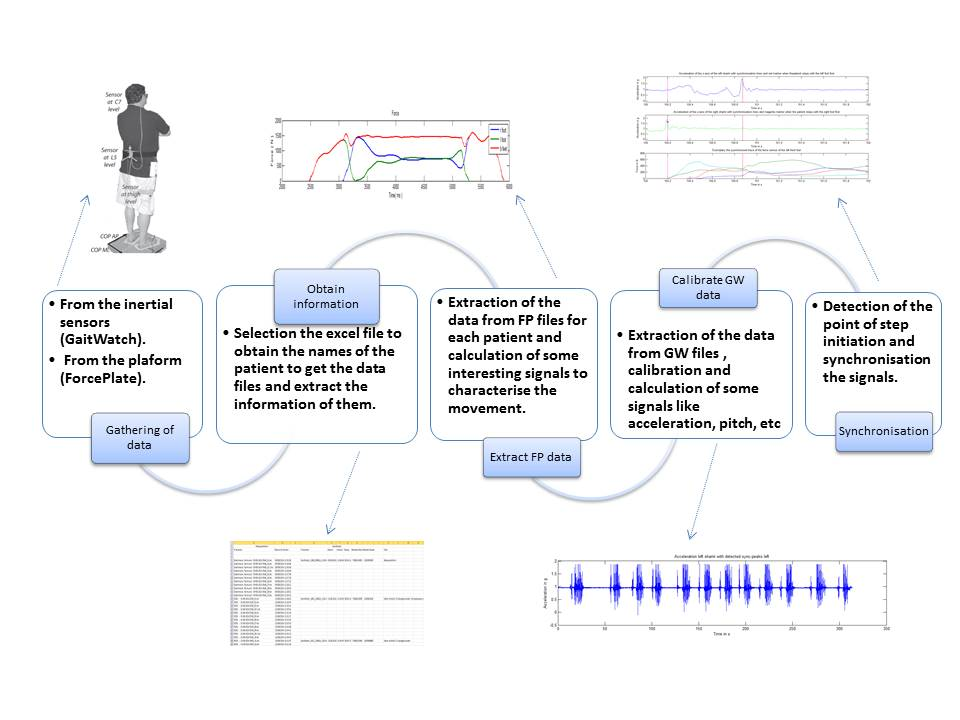
\epsfig{file=imagenes/diagramSynchronisation, width=8cm}
	\caption{Diagram of the Synchronisation's progress.}
	\label{fig:arte1}
\end{figure}

\subsection{Design of developed code  in Matlab}
\subsubsection{Selection, reading and obtaining of information from the excel file}
All patients data , that is, the different files have been generated after the gathering (  of the force plate as well as Gait Watch), gathering date, duration of the experiment and other observations are saved in a Excel file. 

In order to automate all as much as possible, the code is in charge of extraction of the necessary data (files names) to carry out the appropriate calculations for each patient. This is done once the Excel file has been selected, thus, it have to have a specific structure to be able to read the data correctly.

At the end of this fraction of code, we save all file names of both systems (force plate and Gait Watch) corresponding to each patient, in order to access and extract them posteriorly.

\subsubsection{Extraction of the forceplate data}
As we said before, the  force plate data files are recorded independently each others, that is, there is a *.txt file for each repeat.
Each file contains the force data of the toes and heels of both feet. It really realises a distribution of the sensors to cover these four segments. Every measure is obtained for each point of time according to the sample frequency. Also, this file contains the force data from each cell that is part of platform in each frame.

Once we recover this data, some parameters are calculated for the movement characterization carried out over the platform. 

\begin{itemize}
	\item \textbf{Midline}: it represents the midline between both feet. This is important to find the gap between feet and it gives us a idea of their position in the platform. Thus, we carry out the sum of cells force in the anterior-posterior direction. So, this line is in the minimum between two maximum corresponding to the position of both feet. We use this parameter to calculate the center of pressure.
	
	\item \textbf{The total force in the platform for each point of time}: This signal is useful to do the synchronisation due to we can determine clearer when the patient touches the plate.
	
	\item \textbf{Antero-posterior COP}: center of pressure forward-backward direction.
	
	\item \textbf{Medio-lateral  COP}: center of pressure  in right and left direction.
	
	
\end{itemize}

Center of pressure can be expressed as follows:

\begin{equation}
	\label{COP}
	R=\sum_{i}^{n}m_{i}r_{i}
\end{equation}


Where R is the “Center of pressure”, M is the total force and mi are the force that are located in space with coordinated ri, in this case, in the plane. This location (ri) is calculate with respect to the midline.

These signals help us to characterise Anticipatory Postural Adjustments  before gait.  APAs indicate the movement or swinging of body before walk or carry out some movement. Thus, these are the interesting  measures to compare between each repeat as well as each patients to characterise the movement, determine if there is a pattern and figure out the differences and similarities between them.

All these signals are saved for each cycle in a single variable corresponding to the patient.


\subsubsection{Calibration of the GaitWatch data}
When we are working with sensors, calibration is one of the most important aspect that needs to be carried out. Prior to the calibration process,
the information at the sensors  will be a signal composed of integer
numbers  or real numbers bounded into a range which is determined by the precision of the sensors and converters. These numeric values lack of physical value, so it is absolutely necessary to convert them into a scale that can be measured in physical units.

The sensors present several errors due to some effects like scale factor may not be linear or the triad isn’t perfectly orthogonal. To remove these undesired effects, the software include a model to compensate this before the calibration. 
To do so, we have used the code made by Dr. Alberto Olivares Vicente in his doctoral thesis, with minor modifications of his work.

Besides the unwanted effects mentioned above, the output of magnetometers is distorted by wide band measurement noise appearing several large peaks of noise in the signals. To remove this automatically, we used a threshold considering that these peaks are much greater than the mean of the signal.


The erroneus values in the magnetometer signal are removed sustituting these samples by the subsequent value unless the erroneous value is in the last position of the singal, in which case it is substituted by the preceding value.

\subsubsection{Synchronisation}	
In this section we will explain how we carried through the synchronisation of the Force Plate and GaitWatch signals and the considerations adopted to do it properly.

The first step is to detect when the step happens in both systems. In order to do this, we’ll use the completed force from force plate system and shank acceleration from the Gait Watch accelerometer. We chose these signals because it’s easy to see in them the point when the patients step.

The time point when the patient do the step in the platform is exactly when the person touches it, that is, the time point that corresponding with the first sample in the force signal with a value other than zero.

In the acceleration signal case, this fact happens in the first positive peak after a negative peak. The reason is that when patient does a step, the first movement is to rise the leg, so the acceleration vector points downwards thus the great negative peak will be when the leg is in the máximum distance from ground. The immediate movement is to lower the leg and touch the platform, so when the patient puts his leg in the force plate there is a positive peak due to the acceleration vector is pointing upward.

Once we understand the signal behaviour in connection with the patient movement we have to differentiate each cycles in the signal because we have all repeats together in the same file. To do this, we used activity detection code implemented by Dr. Alberto Olivares Vicente in his Doctoral thesis. Figure XX shows the result.

In addition we did a comparative study testing two different methods based on the  computation of the spectrum (Fourier Transform) of the input signal. Also, we tried several input signal to determine which is the best option to do the motion detection in this case.

We will use the Long Term Spectral Detector (LTSD) \cite{Ramirez2004} and a variation of this called Framed Spectrum Detector (FSD). Spectrum-based methods have been used in others kinds of applications like Voice Activity detection \cite{Ramirez2006}\cite{Ramirez2007} and activity sequences detection such as running or sitting-standing up\cite{A.Olivares2013} .

The technical difference between LTSD and FSD is that the first of them compute the Long term spectral Envelope whereas FSD uses the spectrum of each frame  in which the input signal is divided\cite{A.Olivares2013}. What we observe when we use them in our signals is that the results are better when we use LTSD instead of FSD method  in the most of the cases[figure]. 

The LTSD method has a better decision rate than FSD method because it is designed to work under condition where the SNR is low, i.e the signal present large noise\cite{A.Olivares2013}. In our case, we want detect the differents cycles that corresponding to each repeat so the different peaks of activity inside each period can be a problema to do the detection correctly because really it is interpreted like noise for the detector. Thus, the LTSD method is more interesting for this type of signal.

Once we select the best method for the detection we tested several input signal for the detector: shank acceleration signal, absolute value of the shank acceleration signal and module of the shank acceleration signal. Finally, the best result was obtained when we used module of the shank acceleration signal because when this input signal is used in the resulting output signal is easier to distinguish the different episodes.

Furthermore, the motion activity detection was carried out for the right leg as well as left one. It is not necessary in some cases when the patient does the movements or activities quickly since the detected activity interval  include both movements in the same episode. However, when patient waits some time to step again in the same repeat, it is possible that some step is not  include in the interval thus the result would be erroneous. Therefore, to realise a general algorithm useful in whatever case we differentiate between both feet.


Now, we have to consider others aspects like the limbs with which the person start to walk. To do all more comfortable for the patients, it was not specified with which leg they had to do the first step, so we have to determinate automatically this fact. To realise this we calculate all interesting peaks in the right shank acceleration as well as left shank acceleration. Then, we identify first peak in time.

Other important aspect is to consider the sample frequency. The sample frequency is 120 Hz in force plate signals and 200 Hz in GaitWatch signals. Thus, we have to reshape the Force Plate signals to match other signals.

All the key parameters and signals are saved using “time series”  for adding descriptive information to the fact.

Finally, we compare the peak detection for the synchronisation between the accelerometers signal and the gyroscopes signal. The behaviour of the gyroscope signal is very similar to prior signal however this is clearer to the naked eye.
Nevertheless, the correlation between the peaks detected with both systems are almost the same. This indicates that it was done correctly and these detected points are suitable to do the synchronisation.

In XX table we can see that the mean of the difference between the peaks detected with the accelerometer and gyroscope signals is less than 0.5 second in all cases, so it is very small. Also, the correlation between them is very high and the probability of no correlation is smaller than 0.05 what want to say that the correlation is significantly different from zero.

\begin{table}[h]
	\caption{Comparation between the peaks detected with acceletometer and gyroscope}	
	\centering
	\begin{tabular}{|c|c|c|c|}\hline
		
		Patient 				& Average peaks difference 	& Corr 	& Prob 	\\ \hline
		ES39 & 0.3438			& 1.0									& 1.096 e-13					\\
		RK55	& 0.3014			& 1.0									& 2.720 e-13				\\
		RS46o & 0.2500			& 1.0									& 2.750  e-29					\\
		MM57	& 0.4970			& 1.0									& 3.480 e-26					\\
		WS42  & 0.3990			& 1.0									& 1.410 e-25					\\
		SW47	& 0.3615			& 1.0									& 2.190 e-25					\\
		TS40  & 0.2674			& 1.0									& 1.559 e-31				\\ \hline
	\end{tabular}
	\label{tab:comparationAccGyro}
	
\end{table}



\section{APA analysis}
\subsection{Introduction and chapter's structure}

Anticipatory postural adjustments (APAs)  represents balance control that help to stabilise and mobilise the body based on anticipation of forces accompanying voluntary movement such as volitional lifting of the foot during step initiation \cite{Mancini2010} . Step initiation requires a tight proprioceptive coordination between motor commands for postural adjustments and for stepping, so APAs act to accelerate the center of pressure over the stance foot immediately prior to gait \cite{Mancini2009} .

APAs, before gait initiation, are bradykinetic in advanced Parkinson’s disease and may be one of the factor associated with ‘start hesitation’ \cite{Mancini2009} .

Early identification in patients with PD is important because new neuroprotective medications are being tested to slow the progression of this disease and it is necessary to begin early in the disease, prior to significant loss of neurons \cite{Mancini2012} . 

Currently, the most common way to evaluate postural control in the clinic is to use clinical rating scales that are limited by clinician bias, insensitivity to mild impairments and poor reliability. These limitations are serious problems for clinicians and researchers who want to monitor the disease progression, determine intervention efficacy or treat people with mild balance deficits \cite{Mancini2012} .

Technology avaiable for clinicians and researchers to mesure APAs is generally force plate for the analysis of center of pressure. However, force plate is quite large and expensive and requires a proper installation that may not be practical for clinical use. Thus, Body-worn accelerometers have been proposed as a portable, low-cost alternative to a force plate for measurements of postural sway\cite{Mancini2012} .
 
Therefore, along this chapter we will do a comparative study of the measurements obtained of the force plate as well as accelerometers that make up the Gait Watch system. Also, we will compare these measurements with gyroscopes data that form part of this system too, in order to determine what sensors give us the more accurate results.


\subsection{Results discurssion}
